\documentclass[iop]{emulateapj}
\usepackage{color}
\usepackage{natbib}
\usepackage{amsmath}
\bibliographystyle{apj}

\newcommand{\vdag}{(v)^\dagger}
\newcommand{\myemail}{eogorma@tcd.ie}

\shorttitle{BETELGEUSE'S WIND ACCELERATION REGION}
\shortauthors{O'GORMAN ET AL.}

\begin{document}

\title{MULTI EPOCH SPATIALLY RESOLVED RADIO OBSERVATIONS OF BETELGEUSE'S WIND ACCELERATION REGION}


\author{Eamon O'Gorman\altaffilmark{1}, Graham M. Harper\altaffilmark{1}, Alexander Brown\altaffilmark{2}, and Anita M. S. Richards\altaffilmark{3}}
\altaffiltext{1}{School of Physics, Trinity College Dublin, Dublin 2, Ireland}
\altaffiltext{2}{Center for Astrophysics and Space Astronomy, University of Colorado, 389 UCB, Boulder, CO 80309, USA}
\altaffiltext{3}{Jodrell Bank Centre for Astrophysics, School of Physics and Astronomy, University of Manchester, Manchester M13 9PL, UK}

%\email{eogorma@tcd.ie}
%\email{graham.harper@tcd.ie}
%\email{alexander.brown@colorado.edu}
%\email{a.m.s.richards@manchester.ac.uk}


\begin{abstract}
We present multi-epoch spatially resolved radio continuum observations of Betelgeuse at various combinations of wavelengths between $0.7-20.5$\,cm.  We used the Very Large Array (VLA) in the A configuration with the Pie Town (PT) Very Long Baseline Array (VLBA) antenna to fully resolved its atmosphere at 0.7, 1.3, 2.0, and 6.0\,cm at all epochs, and provide flux measurements at 20.5\,cm.

Our low-frequency observations confirm the multiple outburst interpretation of the spectral index differences at high frequencies.

 New multi-epoch e-MERLIN data are urgently required. Betelgeuse's inner atmosphere has undergone a major morphological change in the past 10 years.

\end{abstract}

\keywords{Radio continuum: stars --- Stars: supergiants --- Stars: individual ($\rm{\alpha}$ Ori) --- Stars: mass-loss --- Stars: winds, outflows}

\section{INTRODUCTION}
Red supergiants (RSGs) lose mass to the interstellar medium in the form of a massive ($\dot{M} \sim 10^{-7} - 10^{-4}\,M_{\odot}\,\rm{yr}^{-1}$) cool wind, with terminal velocities ($10\lesssim v_{\infty}\lesssim 50\,{\rm{km}}\,\rm{s}^{-1}$) typically less than the photospheric escape velocity  ($v_{\rm{esc}} \sim 100\,\rm{km}\,\rm{s}^{-1}$). These winds are major contributors of heavy elements to the interstellar medium (ISM) and play a crucial role in stellar evolution \citep{chiosi_1986}, and also in explaining the frequency of supernovae in the galaxy \citep[e.g.,][]{van_loon_2010}. Despite their importance, the mechanisms responsible for the formation of these winds in late K and early M-type RSGs remain largely unknown. Dust is observed too far from the star to play a significant role in the mass-loss process \citep{danchi_1994} and pulsation amplitudes are too low to initiate the mass-loss \citep{smith_1989}. Magnetohydrodynamic (MHD) waves \citep[e.g.,][]{thirumalai_2012} and large convective cells \citep[e.g.,][]{josselin_2007} have been proposed as alternative potential mass-loss mechanisms in RSGs but spatially resolved multi-epoch observations of RSGs are required to test these competing theories.

\subsection{Tracing Betelgeuse's Mass Loss History}
Betelgeuse ($\alpha$ Ori, M2Iab) is the closest isolated RSG \citep[$d=197 \pm 45$\,pc;][]{harper_2008} and is therefore the prototype of the late K and early M spectral type RSG class. Its large angular diameter ($\phi _{\star} = 42.49 \pm 0.06\,$mas in the K band, \citealt{ohnaka_2011}) coupled with its extended atmosphere makes its an excellent target for detailed multi-wavelength studies aiming to build a complete understanding of mass-loss in RSGs. Such studies have recently been carried out and have traced the ejected material over various spatial scales between the ISM and the photosphere. The wind-ISM interaction produces a multi-arc bow shock structure \citep{decin_2012} and a detached H\,I shell elongated in the south-west direction \citep{le_bertre_2012}. Two distinct flows in its circumstellar envelope (CSE) were imaged at 1.3\,mm by \cite{ogorman_2012} which traced CO($J=2-1$) on scales between $\sim 40$\,R$_{\star}$ and $\sim 750$\,R$_{\star}$. These observations revealed an irregular CSE with a notable asymmetry in the south-west direction extending out to $\sim 200$\,R$_{\star}$. Thermal infrared images using the Very Large Telescope (VLT)  uncovered an envelope of inhomogeneous surface brightness up to 100\,R$_{\star}$, whose spectral energy distribution is typical of oxygen-rich dust \citep{kervella_2011}. These images also uncovered a ring-like structure at radius $20-45$\,R$_{\star}$ which may be related to the dust condensation radius. The inner CSE  was probed in the near-infrared with the VLT by \cite{kervella_2009} who discovered a molecular plume extending out to almost 6\,R$_{\star}$ in the south-west direction, which they attributed to the action of a photospheric giant convective cell. Indeed, the photospheric bright spots detected on Betelgeuse by \cite{Haubois_2009} have now been attributed to presence of giant convective cells \citep{chiavassa_2010}. However, this does not provide definitive evidence that such convective cells are actually responsible for initiating the mass-loss.

\subsection{Betelgeuse at Centimeter Wavelengths}
Thermal free-free centimeter continuum emission directly probes the chromospheres and wind acceleration regions of RSGs; the regions identified as the most important for studies of mass-loss mechanisms in evolved stars \citep{holzer_1985}.  The first detailed study of Betelgeuse at centimeter wavelengths was carried out with the Very Large Array (VLA) by \cite{newell_1982}. The source was unresolved but the radio emission was interpreted as chromospheric in origin and extending from $1-4$\,R$_{\star}$. This was in agreement with the Alfv\`en wave models to follow \citep{hartmann_1984} and later Hubble Space Telescope (\textit{HST}) spatially resolved ultraviolet observations \citep{gilliland_1996,uitenbroek_1998}. Spatially resolved VLA plus Multi-Element Radio Linked Interferometer Network (MERLIN) observations at 6\,cm also confirmed the extended nature of the radio emitting region \citep{skinner_1997}. 

\cite{lim_1998} used the VLA in its most extended (i.e., A) configuration to resolve Betelgeuse's atmosphere at 0.7\,cm and partially resolve it at 1.3, 2.0, 3.6, and 6\,cm. Because the radio emission is thermal and optically thick, they were able to calculate the mean gas temperature as a function of radius and discovered that the mean gas temperature never reached chromospheric values (i.e., $\gtrsim 5000\,$K) but decreased steadily from $\sim$3450\,K at 2\,R$_{\star}$, to $\sim$1370\,K at 7\,R$_{\star}$. They also detected an asymmetry in their 0.7\,cm image which they attributed to the action of a large convective cell. To reconcile their results with the extended ultraviolet observations, which probed the same regions, they concluded that the inner atmosphere must be inhomogeneous to accommodate the hot chromospheric plasma, but that the cooler gas must be 3 orders of magnitude more abundant. \cite{harper_2006} used observations of the chromospheric tracer C II] $\lambda 2325\,$\AA to confirm this low filling factor for the chromospheric gas. 

%have a 24$\sigma$ difference between their peak flux densities,
Recently, an unexpected new discovery by \cite{richards_2013} with e-MERLIN, has revealed that two unresolved radio features dominate the total flux density at 5.2\,cm. The two ``radio hotspots'' are separated by $90\pm 10$\,mas (i.e., $\sim 4\,$R$_{\star}$) and have gas temperatures $T_{\rm{e}} \geq 3800\pm 500\,K$ and $T_{\rm{e}} \geq 5400\pm 600\,K$, with the later value significantly above the photospheric temperature ($T_{\rm{eff}}=3690\pm 54\,$K, \citealt{ohnaka_2011}). The features are so extended that they presumably have either momentum or support and are probably connected with the mass-loss mechanism in Betelgeuse. The potential importance of these radio hotspots has been the motivation for this paper. In the following sections we present, analyze, and discuss multi-epoch, mutli-wavelength radio observations of Betelgeuse, taken $\sim 10$ years prior to the e-MERLIN observations. At short wavelengths, our data has comparable or superior resolution to the e- MERLIN data and so the goal of the paper is to search for signatures of these features to improve our understanding of Betelgeuse's wind acceleration region.

\section{OBSERVATIONS AND DATA REDUCTION} 
Betelgeuse was observed with the NRAO\footnote{The National Radio Astronomy Observatory is a facility of
the National Science Foundation operated under cooperative agreement by Associated Universities, Inc.} VLA  in the A configuration with the Pie Town (PT) Very Long Baseline Array (VLBA) antenna at multiple epochs between December 2000 and October 2004. The PT antenna is located 50\,km from the center of the VLA, and its inclusion to the A configuration enhances the east-west resolution by a factor of 2. Our observations are summarized in the first two columns of Table \ref{tab1}. Our two multi-wavelength data sets in 2002 (Program: AH0778) were taken only $\sim 2$ months apart and consist of all wavelength bands between 1.3 and 20.5\,cm. We observed the star again under program AH0824 in 2003 and 2004 at all wavelength bands between 0.7 and 20.5\,cm. We also obtained VLA A configuration plus PT antenna data from the NRAO data archive (Program: AL0525) at  0.7 and 1.3\,cm which were taken in late 2000 and early 2001, respectively.

We used the ``fast switching'' phase calibration technique at 0.7 and 1.3\,cm to compensate for tropospheric phase variations. This allowed us to switch between observations of the point source phase calibrator 0532+075 and Betelgeusese, with cycle times of $2-3$\,min at 0.7, 1.3 and 2.0\,cm. The archival data from 2000/2001 also implemented the fast switching technique at these wavelengths but used the point source phase calibrator 0552+032, which was $\sim 10$ times more faint at 0.7\,cm but 1.4$^{\circ}$ closer to Betelgeuse. We again used interleaving observations of 0532+075 to calibrate phase variations at longer wavelengths, but implemented longer cycle times of $10-20$\,min. Absolute flux calibration was obtained from 3C\,48 at 6.1\,cm, and 3C\,286 at all other wavelengths. The absolute flux density uncertainty is estimated to range from 5\% to 10\% between the longest to shortest wavelengths, respectively. The flux density error values quoted in the remainder of this paper do not include this systematic error but represent the $\pm 1\sigma$ value. The raw visibilities were flagged and calibrated according to standard VLA continuum data reduction procedures using the Astronomical Image Processing System \cite[AIPS;][]{greisen_1990}. The calibrated visibilities were imaged in both AIPS and the Common Astronomical Software Application  \cite[CASA;][]{mcmullin_2007} package.


\begin{deluxetable*}{lcccccccc}
\tabletypesize{\scriptsize}
%\tablecolumns{6} 
%\tablewidth{0pt} 
\tablecaption{Multi Epoch VLA A Configuration Plus PT Link Observations of Betelgeuse.}
\tablehead{\colhead{Date}						&
			\colhead{Wavelength}			    &
           	\colhead{Restoring Beam}            &
           	\colhead{Image rms}            		&
           	\colhead{$\theta _{\mathrm{maj}}$}  &
			\colhead{$\theta _{\mathrm{min}}$}	&
           	\colhead{P.A.}  &
          	\colhead{$F_{\nu}$}  &
           	\colhead{$T_{b}$}  \\
	\colhead{}		                			& 
	\colhead{(cm)}                         		& 
	\colhead{(mas $\times$ mas)}   	&
	\colhead{(mJy/Beam)}                    	&
	\colhead{(mas)}   		    &
	\colhead{(mas)}   		    &
	\colhead{(deg)}   		    &
	\colhead{(mJy)}   		    &
	\colhead{(K)}		}
\startdata
		 2004 Oct 21,30  & 0.7 & $39\times 26$ & 0.37	& $99\pm 3$ & $92 \pm 20 $& $92\pm 20$ &$28.68\pm 0.53$ & $2940\pm 170$\\
		 				 & 1.3 & $80\times 42$ & 0.09   & $127\pm 2$& $ 114\pm 4$ & $85\pm 5$& $13.83\pm 0.10$& $3140\pm 80$\\
						 & 2.0 & $121\times 91$ & 0.08  & $158\pm 6$& $ 152\pm 17$ & $132\pm 59$ & $7.23\pm 0.15$& $2270\pm 130$ \\
						 & 3.6 & $208\times 126$ & 0.02	& $215\pm 7$& $188\pm 15$ & $0\pm 10$& $3.34\pm 0.03$& $2110\pm 110$\\
						 & 6.1 & $377\times 264$ & 0.02	& $314\pm 30$& $204\pm 54$ & $0\pm 20$ & $1.55\pm 0.04$& $1140\pm 160$\\
						 & 20.5& $1262\times 889$ & 0.03& $< 889$ & $< 889$ & $\dots$ &$0.25\pm 0.03$ &$ \textgreater 260$\\
\hline
\rule{-2.6pt}{2.5ex}  2003 Aug 10,12 & 0.7 		& $40\times 27$ & 0.46	& $103\pm 4$& $92\pm 10$ & $104\pm 16$& $28.05\pm 0.84$& $2760\pm 230$ \\
									 & 1.3		& $80\times 42$ & 0.17	& $122\pm 5$& $115\pm 12$& $0\pm 5$& $11.20\pm 0.24$& $2490\pm 150$\\
									 & 2.0		& $119\times 96$& 0.10	& $132\pm 10$& $ 116\pm 22$& $11\pm 27$& $5.88\pm 0.17$&$3040\pm 360$\\
									 & 3.6		& $ 204\times 139$&	0.03& $193\pm 7$& $ 141\pm 17$ & $152\pm 7$& $2.80\pm 0.04$&  $2610\pm 170$\\
									 & 6.1 		& $378\times 297$&	0.03& $247\pm 47$& $180\pm 103$ & $169\pm 28$& $1.22\pm 0.04$&$2040\pm 680$ \\
					                 &20.5		& $1247\times 931$&0.04	& $< 931$& $< 931$ & $\dots$& $0.26\pm 0.03$& $ \textgreater 250$\\
\hline
\rule{-2.6pt}{2.5ex}  2002 Apr 12,13  & 1.3 		& $91\times 59$ & 0.18	&$134\pm 9$ & $102\pm 16$& $36\pm 10$& $8.96\pm 0.24$& $2170\pm 250$\\
							& 2.0		&$131\times 98$ & 0.39	& $166\pm 16$& $105\pm 27$&$41\pm 11$ & $5.32\pm 0.24$& $2420\pm 450$ \\
							& 3.6		& $224\times 155$&0.03	& $234\pm 9$& $171\pm 18$& $41\pm7$& $2.66\pm 0.04$& $1690\pm 110$\\
							& 20.5	& $1398\times 1146$& 0.06	& $< 1146$ & $< 1146$ & $\dots$& $0.38\pm 0.06$& $ \textgreater 240$\\
\hline
\rule{-2.6pt}{2.5ex}  2002 Feb 17,18 & 1.3 		& $83\times 48$&0.14	&$120\pm 4$ & $109 \pm 8$& $31\pm 13$&$10.87\pm 0.17$ & $2750\pm 140$\\
									& 2.0		& $128\times 90$&0.11	&$140\pm 13$& $136\pm 33$& $0\pm 28$&$5.38\pm 0.22$ & $2150\pm 300$\\
									& 3.6		& $200\times 135$&	0.03&$217\pm 9$ & $182\pm 21 $& $ 0\pm 5$ & $2.85\pm 0.04$& $1830\pm 110$\\
									& 20.5		&$1312\times 951$ &0.05	& $< 951$& $< 951$& $\dots$& $0.30\pm 0.05$& $ \textgreater 270$\\
\hline
\rule{-2.6pt}{2.5ex}  2001 Jan 02  & 1.3 		& $78\times 42$&0.08	&$124\pm 2$ & $114\pm 4$& $40\pm 8$& $12.58\pm0.08$& $2920\pm 70$ \\
 		 2000 Dec 23 & 0.7		& $44\times 20$& 0.18	&$98\pm 2$ &$90\pm 4$ &$0\pm 8$ & $29.02\pm 0.30$& $3070\pm 100$
%\hline
%\rule{-2.6pt}{2.5ex}  1998 Mar 29,30 & 0.7 		& &	& $104\pm 6$& $0.88\pm 0.07$& $118\pm 20$& $18.19\pm 0.73$& $1770\pm 180$ \\
%									 & 1.3		& & 	& $157\pm 8$ & $0.61\pm 0.06$& $46\pm 6$&$10.99\pm 0.31$ & $2420\pm 250$
\enddata
\tablenotetext{}{Notes.- The restoring beam sizes and image rms noise values are taken from the uniformly weighted radio maps that include the PT antenna baselines. The position angles (measured in degrees east of north) of the restoring beams are not quoted here, but are all between $30^{\circ}$ and $70^{\circ}$. The major and minor axis of the stellar radio disk $\theta _{\mathrm{maj}}$ and $\theta _{\mathrm{min}}$, the position angle P.A., and the total flux density $F_{\nu}$, are all derived from the best-fit uniform-brightness ($T_b$) elliptical-disk models.}
\label{tab1}
\end{deluxetable*}

\subsection{Imaging}\label{obs2.1}
The calibrated visibilities at all wavelengths were imaged using CASA's \textit{clean} task while applying uniform weighting. With uniform weighting, each visibility is given a weight that is inversely proportional to the sampling density function. This optimises the full resolution of the array and minimises the sidelobe level. However, it also leads to an increase in the image noise level in comparison to natural weighting, which gives a constant weight to all visibilities, and Briggs weighting, which is a compromise between uniform and natural weighting. Additional images were also created at 0.7 and 1.3\,cm which implemented both Briggs weighting, and natural weighting with a restoring beam size equal to that obtained using uniform weighting, as used in \cite{lim_1998}. These additional images were used to check if asymmetries produced by one weighting scheme could be reproduced by another.

\subsection{Calibrated Visibilities}
Betelgeuse's position was initially offset by a few restoring beams from the interferometer phase center to avoid any possible spurious artefacts which might accumulate there. One such artefact was noticed in the 2.0\,cm image from April 2002 but our target was sufficiently far away and was not contaminated. We fitted elliptical Gaussian brightness distributions to the source at each wavelength and epoch and measured the position of the peak emission. We then used CASA's \textit{fixvis} task to shift the visibilities such that this peak emission position was placed at phase center. The Python-based task \textit{uvmultifit} \citep{marti_vidal_2014} was then used to fit elliptical disks to the calibrated visibilities, with the major axis ($\theta _{\rm{maj}}$), axis ratio ($\theta _{\rm{min}}/\theta _{\rm{maj}}$, where $\theta _{\rm{min}}$ is the minor axis), position angle (P.A.), and flux density ($F_{\nu}$) left as free parameters. We bounded the axis ratio between 0 and 1, and the position angle between 0 and 180$^{\circ}$.

\section{RESULTS} 
\subsection{Radio Maps}
Radio maps were produced at all wavelengths using uniform weighting to utilize the full capabilities of the PT baselines and achieve maximum spatial resolution. The corresponding restoring beam sizes and image rms noise levels are provided in columns 3 and 4 of Table \ref{tab1}. Calibrations issues with the two 6.1\,cm data sets from 2002 resulted in rms noise values being ~10 times higher than expected. This resulted in the source not being detected in the April 2002 map and the source being located $\sim 300$\,mas away from its expected position in the February 2002 map. We therefore do not include these 6.1\,cm results in Table \ref{tab1} and in any of the analysis.The remainder of the maps were generally of excellent quality with the source clearly resolved at the shorter wavelengths. No deviations from axially symmetry were present in any of the maps between 1.3 and 20.5\,cm.

All of the 0.7\,cm maps showed significant deviations from axial symmetry. However, when the data sets were imaged using the different weighting schemes described in Section \ref{obs2.1}, the morphology was inconsistent. For example, the maps created using standard uniform weighing were morphologically different to the maps created using natural weighting with a restoring beam of size corresponding to that produced with uniform weighting. These inconsistencies are probably due to poor phase stability resulting from rapid tropospheric phase fluctuations of which our cycle times were not short enough to compensate for. To investigate this further, we removed the PT antenna baselines and again imaged the data using the two aforementioned
imaging techniques. We found that two data sets (i.e., from 2000 and 2004) produced images that had consistent morphology when any of the imaging techniques were applied. The observing logs of the other data sets report poorer weather conditions in agreement with our imaging analysis. The resulting images are plotted in Figure \ref{fig1} along with the 0.7\,cm image from \cite{lim_1998} for comparison. In these data sets, the cycle time was adequate to obtain reasonable phase transfer from the calibrator to the source but shorter cycle times were probably required for the other data sets due to poorer weather. Unlike the \cite{lim_1998} map, no asymmetries are present in either of our two maps as is clearly evident in Figure \ref{fig1}. These maps indicate that large scale asymmetries are not always present in Betelgeuse's inner atmosphere.

\begin{figure*}
\mbox{
\includegraphics[trim = 6mm 0mm 0mm 0mm, clip,scale=0.95]{/home/eamon/pietown/paper/figs/fig1.ps}
%\includegraphics[trim = 30mm 90mm 50mm 80mm, clip,scale=0.55]{/home/eamon/pietown/paper/figs/nature_fig.ps}
%\includegraphics[trim = 0mm 50mm 20mm 58mm, clip,scale=0.4,angle=90]{/home/eamon/pietown/paper/figs/vla_q_2000.ps}
%\includegraphics[trim = 0mm 0mm 20mm 58mm, clip,scale=0.40,angle=90]{/home/eamon/pietown/paper/figs/vla_q_2004.ps}
}
\caption{VLA A configuration maps of Betelgeuse at 0.7\,cm over three different epochs. These maps have been created by naturally weighting the visibilities and using a restoring beam corresponding to the size created from uniform weighting. The restoring beam size and shape is located in the bottom left position of each panel while the red circle is the approximate location and size of the optical photosphere. From left to right the beam sizes are x, y, and z$\prime\prime$ and the rms noise values are x, y, and z\,mJy\,beam$^{-1}$. \textit{Left panel}: The \cite{lim_1998} map shows an asymmetry in the east direction. The position of the photosphere is here assumed to be .... \textit{Middle and right panels}: Our 0.7\,cm maps created without any visibilities from the PT baselines. No asymetries deviating from the restoring beam shape are present. The position of the photosphere is here assumed to be located on the peak emission.}
\label{fig1}
\end{figure*}

\subsection{Diameters} 
Importance of working in the visibility domain
Previous VLA observations have only spatially resolved the stellar atmosphere at 0.7\,cm but here we fully resolve the star at all wavelengths between 0.7 and 6.1\,cm. Skinner discussion
Point to Table 1 give diameter variability.

xaxis 'Real Visibility (mJy)' colour pietown baselines

Compare to Harper 2001 paper


\subsection{Flux Densities}
obtained from visibilty fits but also checked against elliptical Gaussian fitted results
plot flux versus frequency (see harper paris presentation)
\subsection{Temperature Profiles}
give more exact lim formula 

\section{DISCUSSION}
\subsection{Radio Flux Density Variability} 
see Reid \& Menton 1996 conf proceedings\\
see Drake conf proceedings\\
e-MERLIN flux is concentrated\\
see Harper\_variability. ps\\
does flux go up as ang diam go up\\
see Harper 2001 discussion

\subsection{Structure of Wind Acceleration Region} 
Thermal structure (Lim vs vs Ours vs e-MERLIN)\\
see Reid \& Menton 1996 conf proceedings\\
Harper model

\subsection{Where are the Hotspots?}

No sign of hotspots (see Harpers pie town proceedings )
See harper 2001 discussion	
emerlin rules out convective cells, magnetic fields?





\section{CONCLUSIONS}
 


\acknowledgments
The data presented in this paper were obtained with the Karl G. Jansky Very Large Array (VLA) which is an instrument of the National Radio Astronomy Observatory (NRAO). The NRAO is a facility of the National Science Foundation operated under cooperative agreement by Associated Universities, Inc. 

{\it Facilities:} \facility{VLA}.



\bibliography{references}

\end{document}
